%!TEX root = ../main.tex

\chapter{Methodology\label{chap:how_to}}

\section{Problem definition}
We will define a domain as a subset of all the possible \ac{MDP} environments.
A standard domain is characterized by a 4-tuple $\mathcal{D} = (S, A, P, R)$ where:

\begin{itemize}
    \item $\mathbf{S:}$ denotes a set of states called the state space.
    \item $\mathbf{A:}$ is the set of actions called the action space.
    \item $\mathbf{P(s'|s, a):}$ is the probability that a given action $a \subset A$, at state $s \subset S$ will lead to a new state $s' \subset S$. 
    \item $\mathbf{R(s',s,a):}$ is the inmediate reward, or expected inmediate reward, recived for transitioning from $s$ to $s'$ after performing action $a$. 
\end{itemize}
From the source domain, $\mathcal{D}_s$, (i.e. simulation), we can control a set of N parameters of the variable aspects of each environment that define a configuration vector, $\vec{\xi} = [\xi_1, \xi_2, ..., \xi_N]$.
Examples of $\xi$ can include:

\begin{tabular}{c|c}

    Physical properties & $\xi_{\text{mass}}, \ \xi_{\text{inertia}}, \ \xi_{\text{drag}}, \ \xi_{\text{gravity}}$ \\
    Perception properties & $\xi_{\text{sensor\_noise}}, \ \xi_{\text{sensor\_latency}}$ \\
    Viual properties & $\xi_{\text{lighting}}, \ \xi_{\text{texture}}, \ \xi_{\text{fov}}$ \\
    Scene properties & $\xi_{\text{gate\_pos}}, \ \xi_{\text{gate\_size}}, , \ \xi_{\text{gate\_num}}$ \\
    
\end{tabular}

Each configuration is sampled from a randomization space, $\vec{\xi} \in \Xi \subset \Re^N$, with a probability distribution $\vec{\xi} \sim p(\vec{\xi})$.
Where the parameters are bounded to be within an interval $\xi_i \in [\xi_i^{\text{low}}, \xi_i^{\text{high}}]$ \cite{weng2019DR}. 

At the start of every training episode, a new environment insance is created by sampling a new configuration vector $\vec{\xi}$ from the distribution $p(\vec{\xi})$. 
Therefore, the agent will interact with a specific \ac{MDP} environment, that is to say, a specific domain $\mathcal{D}_{\vec{\xi}}$. 
This way, the agent can collect data from a vareity of environments that otherwise would reamain unexplored. 
\begin{figure}[H]
  \centering

  \begin{adjustbox}{max totalsize={0.5\textwidth}{0.4\textheight}, center}
    

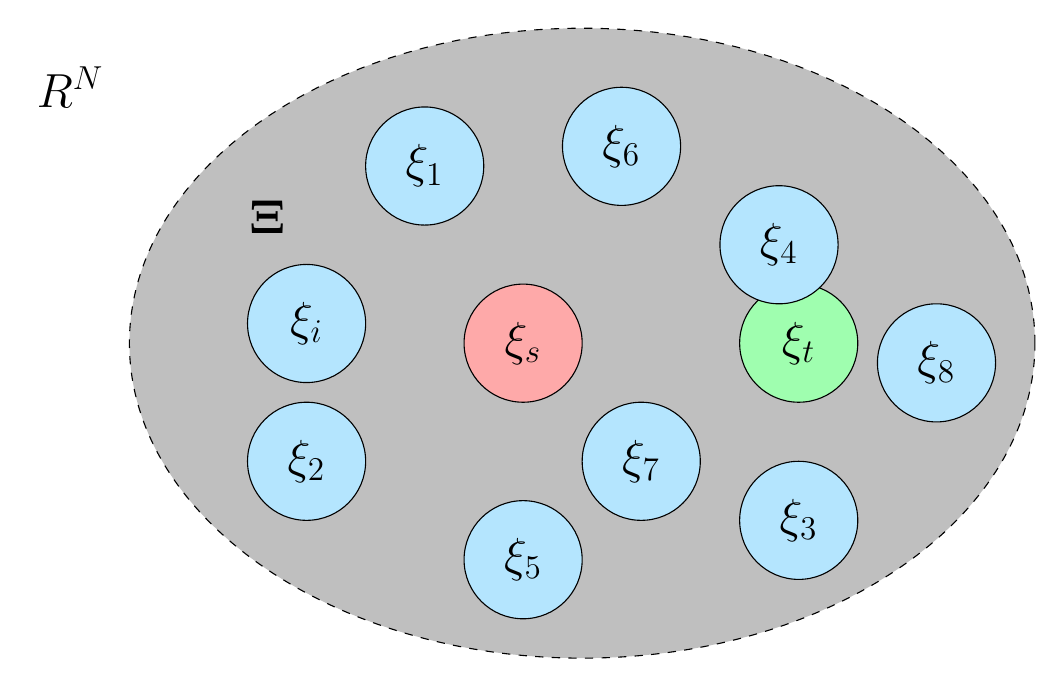
\begin{tikzpicture}[node distance=1cm, auto,]
\tikzstyle{every node}=[font=\LARGE]
\draw [ fill=gray!50, dashed] (8.25,7.75) ellipse (5.75cm and 4cm);
% \draw [dashed] (9.25 ,7.75) ellipse (3.25cm and 2cm);
\draw [ dashed] (14,11.75) ellipse (0cm and 0cm);
\draw [ dashed] (13,11.5) ellipse (0cm and 0cm);
\draw [ fill={rgb,255:red,180; green,229; blue,254} ] (4.75,8) circle (0.75cm) node {\LARGE $\xi_i$};
\draw [ fill={rgb,255:red,159; green,254; blue,175} ] (11,7.75) circle (0.75cm) node {\LARGE $\xi_t$};
\draw [ fill={rgb,255:red,180; green,229; blue,254} ] (6.25,10) circle (0.75cm) node {\LARGE $\xi_1$};
\draw [ fill={rgb,255:red,180; green,229; blue,254} ] (4.75,6.25) circle (0.75cm) node {\LARGE $\xi_2$};
% \draw [ fill={rgb,255:red,180; green,229; blue,254} ] (9.25,9) circle (0cm) node {\LARGE $\xi_3$};
% \draw [ fill={rgb,255:red,180; green,229; blue,254} ] (10,9) circle (0cm) node {\LARGE $\xi_4$};
\draw [ fill={rgb,255:red,180; green,229; blue,254} ] (11,5.5) circle (0.75cm) node {\LARGE $\xi_3$};
\draw [ fill={rgb,255:red,180; green,229; blue,254} ] (10.75,9) circle (0.75cm) node {\LARGE $\xi_4$};
\draw [ fill={rgb,255:red,180; green,229; blue,254} ] (7.5,5) circle (0.75cm) node {\LARGE $\xi_5$};
\draw [ fill={rgb,255:red,180; green,229; blue,254} ] (8.75,10.25) circle (0.75cm) node {\LARGE $\xi_6$};
\draw [ fill={rgb,255:red,180; green,229; blue,254} ] (9,6.25) circle (0.75cm) node {\LARGE $\xi_7$};
\draw [ fill={rgb,255:red,180; green,229; blue,254} ] (12.75,7.5) circle (0.75cm) node {\LARGE $\xi_8$};
\draw [ fill={rgb,255:red,254; green,169; blue,169} ] (7.5,7.75) circle (0.75cm) node {\LARGE $\xi_s$};
\node [font=\LARGE] at (4.25, 9.35) {$\mathbf{\Xi}$};
% \node [font=\LARGE] at (7.75, 9.25) {$\mathbf{\Theta}$};
\node [font=\LARGE] at (1.75, 11) {$\mathbb{R^N}$};


    
\end{tikzpicture}

  \end{adjustbox}

  \caption{Red and green the source and target domains respectively. In blue, differents instances of the randomized source space (all represented domains with the same size, $N$). }
  \label{fig:pgfplots_diagram}
\end{figure}
Hereby, during training, the neural network weights and biases $\theta$ are optimized to maximize the expected reward $R$ across a distribution of randomized domains.
With th objective of finding the optimal, $\theta^*$.
\begin{equation}
    \theta ^* = \arg \max_{\theta} \mathbb{E}_{\vec{\xi}\sim\Xi} \left[\mathbb{E}_{\pi_\theta,\tau\sim D_\xi}[R(\tau)] \right]
\end{equation}


And it will be able to react to certain unseen variations of the randomization space.
More specifically, from the 

% Hereby, the policy will be exposed to a rich varaeity of environments 
% Examples of randomization parameters could include physical properties such as $\xi_\text{mass},\ \xi_\text{inertia},\ \xi_\text{drag}$
\section{Quadcopter model}


\section{\ac{RL} set-up}



\begin{figure}[h]
  \centering

  \begin{adjustbox}{max totalsize={0.5\textwidth}{1.0\textheight}, center}
    \tikzset{
  >=latex, % for default LaTeX arrow head
  node/.style={thick,circle,draw=myblue,minimum size=22,inner sep=0.5,outer sep=0.6},
  node in/.style={node,green!20!black,draw=mygreen!30!black,fill=mygreen!25},
  node hidden/.style={node,blue!20!black,draw=myblue!30!black,fill=myblue!20},
  node convol/.style={node,orange!20!black,draw=myorange!30!black,fill=myorange!20},
  node out/.style={node,red!20!black,draw=myred!30!black,fill=myred!20},
  connect/.style={thick,mydarkblue}, %,line cap=round
  connect arrow/.style={-{Latex[length=4,width=3.5]},thick,mydarkblue,shorten <=0.5,shorten >=1},
  node 1/.style={node in}, % node styles, numbered for easy mapping with \nstyle
  node 2/.style={node hidden},
  node 3/.style={node out}
}
\def\nstyle{int(\lay<\Nnodlen?min(2,\lay):3)} % map layer number onto 1, 2, or 3

\begin{tikzpicture}[x=2.2cm,y=1.4cm]
  \message{^^JNeural network, shifted}
  \readlist\Nnod{4,5,5,5,3} % array of number of nodes per layer
  \readlist\Nstr{n,m,m,m,k} % array of string number of nodes per layer
  \readlist\Cstr{\strut x,a^{(\prev)},a^{(\prev)},a^{(\prev)},y} % array of coefficient symbol per layer
  \def\yshift{0.5} % shift last node for dots
  
  \message{^^J  Layer}
  \foreachitem \N \in \Nnod{ % loop over layers
    \def\lay{\Ncnt} % alias of index of current layer
    \pgfmathsetmacro\prev{int(\Ncnt-1)} % number of previous layer
    \message{\lay,}
    \foreach \i [evaluate={\c=int(\i==\N); \y=\N/2-\i-\c*\yshift;
                 \index=(\i<\N?int(\i):"\Nstr[\lay]");
                 \x=\lay; \n=\nstyle;}] in {1,...,\N}{ % loop over nodes
      % NODES
      \node[node \n] (N\lay-\i) at (\x,\y) {$\Cstr[\lay]_{\index}$};
      
      % CONNECTIONS
      \ifnum\lay>1 % connect to previous layer
        \foreach \j in {1,...,\Nnod[\prev]}{ % loop over nodes in previous layer
          \draw[connect,white,line width=1.2] (N\prev-\j) -- (N\lay-\i);
          \draw[connect] (N\prev-\j) -- (N\lay-\i);
          %\draw[connect] (N\prev-\j.0) -- (N\lay-\i.180); % connect to left
        }
      \fi % else: nothing to connect first layer
      
    }
    \path (N\lay-\N) --++ (0,1+\yshift) node[midway,scale=1.5] {$\vdots$};
  }
  
  % LABELS
  \node[above=1,align=center,mygreen!60!black] at (N1-2.90) {input\\[-0.2em]layer};
  \node[above=1,align=center,myblue!60!black] at (N3-2.90) {hidden layers};
  \node[above=1,align=center,myred!60!black] at (N\Nnodlen-2.90) {output\\[-0.2em]layer};
  
\end{tikzpicture}
  \end{adjustbox}

  \caption{Red and green the source and target domains respectively. In blue, differents instances of the randomized source space (all represented domains with the same size, $N$). }
  \label{fig:nn}
\end{figure}

\section{\ac{DR} configurations}

